%! TEX root = 'main.tex'
\section{Overview}
\label{sec:overview}

Cybersecurity is essential because computing devices encompass almost every respect in people's daily life. It is especially so when the attacks on critical infrastructure emerge. There are many ways to breach a computer system. Software-based attacks are the most common and widespread methods but not necessarily the only way. Operating system and software vulnerability hunting and exploiting, the cracking of authentication methods and protocols have the most forms of attacks and so do their countermeasures.

To perform a conventional cyberattack, the attacker needs to, including but not limited to, join the network, talk the same protocol with the target system, find a service's loophole or vulnerability, and successfully exploit it. The entire virtual path to the system's highest privilege is full of thorns, meaning authentications and exploit mitigations.

The cyberattacks draw most of the attention, and physical attacks are underrated. We roughly make physical attacks into two categories, as we depict them in ~\autoref{fig:bigpic}, sneak attack and supply-chain attack. We try to describe that many control devices such as PLC in a power grid are deployed in remote substations for the sneak attack. It is questionable whether the security of the plant has been improved in the same way. For example, a theft probably needs to crack doors to enter the room where the device is located. However, the commonly used padlock has the same structure as it was decades ago. How to enter a room is out of this paper's scope, but installing a hardware backdoor after physically access a device, we argue, is a real threat.

The supply-chain attack is a hot topic recently due to the SolarWinds incident~\cite{solarwinds}. Even though it has also happened in software, the problem behind this is the same. The pre-installed backdoor penetrates the companies or organizations with benign software and hardware devices.

\begin{figure*}[ht]
	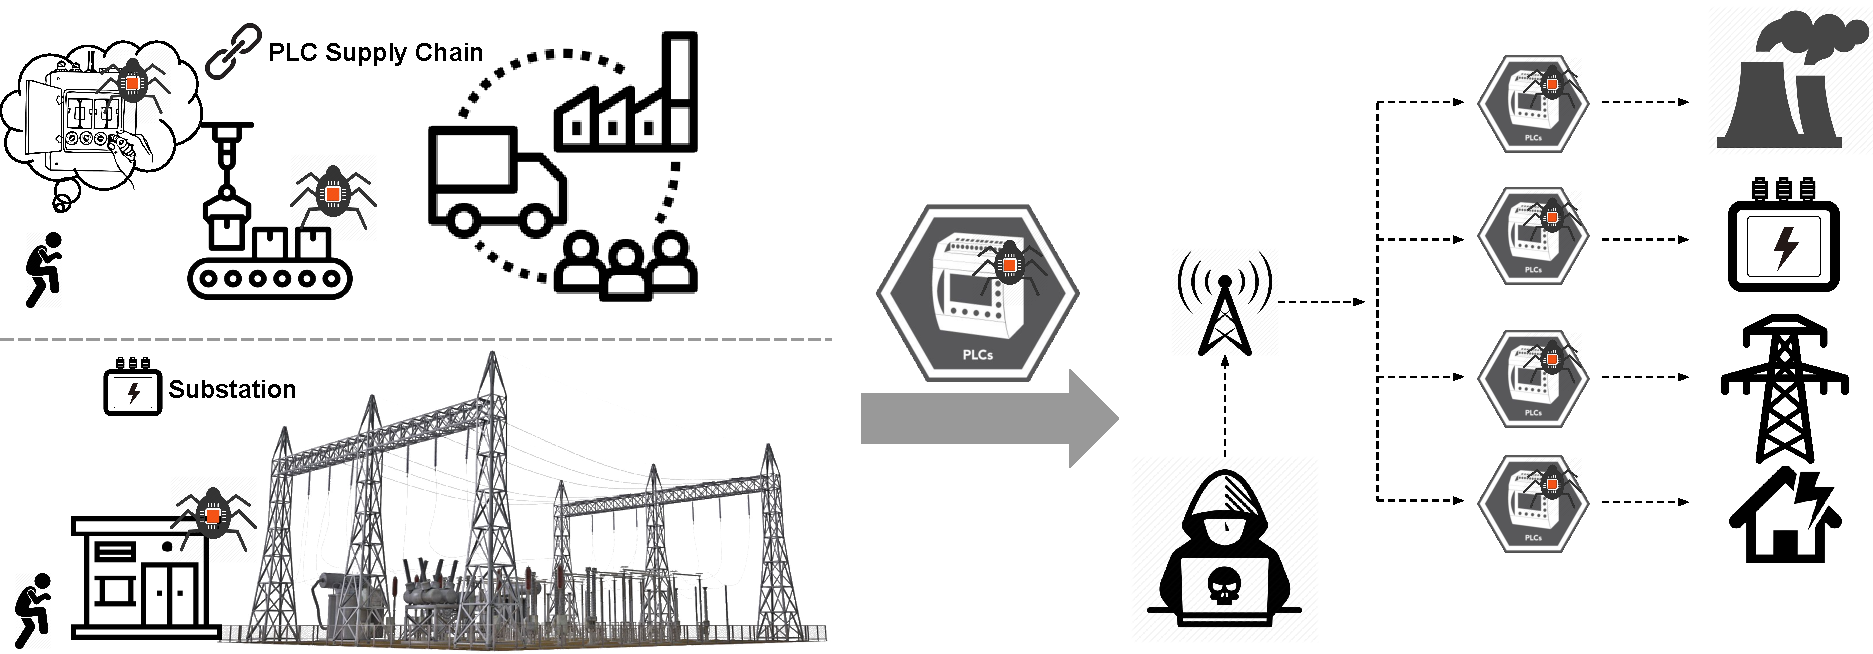
\includegraphics[width=\textwidth]{figures/bigpic}
	\centering
	\caption{Hardware backdoors are installed through industrial control system supply chain penetration of physical contact with industrial systems. Form a botnet that can remotely control multiple points simultaneously.}
	\label{fig:bigpic}
\end{figure*}


When the attacker can control a certain number of PLCs, he can initiate a synchronous attack remotely through the cellular network. In this way, the attacker does not need to tamper with the firmware or update ladder logic, so there is no need to go through the existed mitigations such as security checking and ladder logic emulation.


%\subsection{Adversary Model}
%
%
%
%In general, to compromise an industrial control system, attacks could been categorized into two basic groups. Software exploitation and hardware manipulation.
%
%\textbf{Software Exploitation.} Many attacking surfaces exist in this category. In the past, due to the lack of security measure, attackers can connect to PLC and use the existing mechanism to load a new ladder logic or module to run, \textcolor{red}{cite simens}. Or, there are many network faced services such as CAN bus or a web portal may potentially have vulnerability in their implementation. By exploiting the vulnerabilities, attackers could first win part of the PLC and then further gain control of the real-time microcontroller which directly controls the physical industrial devices \textcolor{red}{cite simens}. These type of attack is straight forward and effective. But the problem is that direct network access is required. Network isolation is a common practice in vital industrial systems. It's still possible to make a successful attack, for instance, the infamous Stuxnet. The Stuxnet virus used several 0day exploits and had a  penetration plan, and it actually took years to spread a virus and finally located the target network. On the other hand, many research focus on this and mitigations start to get applied, which makes direct software exploit more and more difficult. Naturally, leaving preset backdoors in firmware and hardware starts to draw attackers attention.  
%
%
%\textbf{Hardware manipulation.} Hardware attacks are easily related to supply chain security. Every node in the supply chain can be infiltrated and exploited by attackers. Chip design modification is the most stealthy one, but it's hard due to the fact that there are only few microchip fabrication plant can produce certain type of microcontroller or SoC. Lower in the supply chain where the PLC is manufactured and assembled, it's more practice. Detecting a supply chain compromise is a difficult and costly endeavor. This requires strict security and quality control throughout every phase of the supply chain even including shipping.
%
%Firmware modification attacks is effective, even with some lightweight checksum and encryption scheme which can be bypassed. But, if the hardware keeps integrity, then the malicious firmware could be find out by software auditing such as a firmware image trust list.
%
%Hardware have some advantages. When looked at a PCB board of PLC, mostly the electronic design, wire routing is not intuitive for most of the users. Several layers of PCB contains hundreds of wires connecting dozens of chips. And, for each chip, we tend to believe what it prints on the surface. There is no easy to verify the functionality of each chip to what it claims. As mentioned earlier, all the software level logic, to the physical systems, eventually ends up as signals on the GPIO pins. Changing the voltage levels on the wires severs the purpose of controlling industrial devices as what software ladder logic does. There are different peripheral protocols and buses in a PLC, each of them plays different roles in the system. For example, in order to send in data, some flash chip could use SPI as the protocol to communicate with the microcontroller. Tapping on the SPI wires, the malicious circuit could change the data that being transferred. In this paper, we choose a very common interface called JATG as the main carrier of our malicious operations.   
%
%JTAG is is an industry standard for verifying designs and testing printed circuit boards after manufacture. Among various components and buses on a PCB board, JTAG is low speed and it can reach a wide range of the system. Multiple chips can be daisy chained together. This type of setup allows one set of JTAG interface to control multiple devices.
%
%We prototyped a device which is small enough to mount on the PCB board of a PLC. This could happen inside the supply chain, any one with physical access to a PLC could easily open the case and mount the hardware implant.
%
%We also propose a more stealthy way detailed in Further Work section.
\subsection{Adversary Model}

We assume the attacker is aware of what type of PLC the target plant uses, and it is no difficult to purchase one from the market so that the attacker can study the target well before performing the attack.

Inside the PLC case, the PCB boards and the IC chips mounted on top are well exposed. For instance, Chip-on-Board (COB)~\cite{lau1994chip} with the black glob-top makes the IC's pins challenging to identify. Fortunately, high-end microcontroller products rarely use this type of packaging. It would be helpful if the microcontroller has JTAG pins and the JTAG interface is not disabled by programming fusing bits at the factory. Without JTAG, the attacker can still control the IO or modify the firmware image during the transfer from flash chip to RAM. However, these techniques highly depend on the IC chips used in the PLC.

To remotely control the device, the attacker uses a cellular network or WIFI to communicate with the hardware backdoor. Therefore the PLC must not be deployed in an electromagnetic isolation environment where the wireless signal can not transmit outside.

The operating system and software mitigation that runs on the microcontroller does not affect the backdoor.  The system can have the memory protection mechanism based on MMU or MPU, and the derivative mitigation such as \textbf{W}rite $\oplus$ e\textbf{X}ecute.



\subsection{Challenges and Approaches}

The major challenge in attacking PLCs is not having enough information about the device. Some vendors publish the microcontroller's datasheet, but some vendors use proprietary design with highly customized instruction set architecture (ISA).  The layout of the PCB board and the on-board pin definition are also not publicly available.

\textbf{\textit{Firmware.}} The flash chip stores the real-time operating system and the associated file system, referred to as the firmware. Some modules may use a commercial real-time operating system such as VxWorks, but the firmware update's format is confidential and usually protected by encryption verification. Those modules are mostly used to communicate with the host for updates or establish a web server. For the real-time module that we try to control, the type of operating system is unknown.

To solve it, we use the following two ways to read out the firmware. We use the JTAG interface and the CoreSight DAP functionality to read out the flash and ROM memory, which are part of the microcontroller. We also use In-System Programming (ISP) to read the flash chip after the board is powered off.  With the firmware images and reverse engineering effort, we can identify the internal data structures and libraries used to control peripheral devices.

\textbf{\textit{JTAG Pins.}} On some boards, the JTAG pins are difficult to trace, especially when the microcontroller is in BGA packaging where all the pins are underneath the chip. Fortunately, the board we work on has a 10-pin solder pad, as shown in ~\autoref{fig:board_jtag}, which is likely to be the unsoldered JTAG socket. With the microcontroller's datasheet, we can find the chip's JTAG PINs and then use a multimeter to test the continuity between the chip and the pad. It is trivial to identify each pin on the pad.

In our case, the chip supports both JTAG and Serial Wire Debug (SWD)\cite{ashfieldserial}, and some of the pins are shared. We choose to use JTAG in this project.

\begin{figure}[th]
	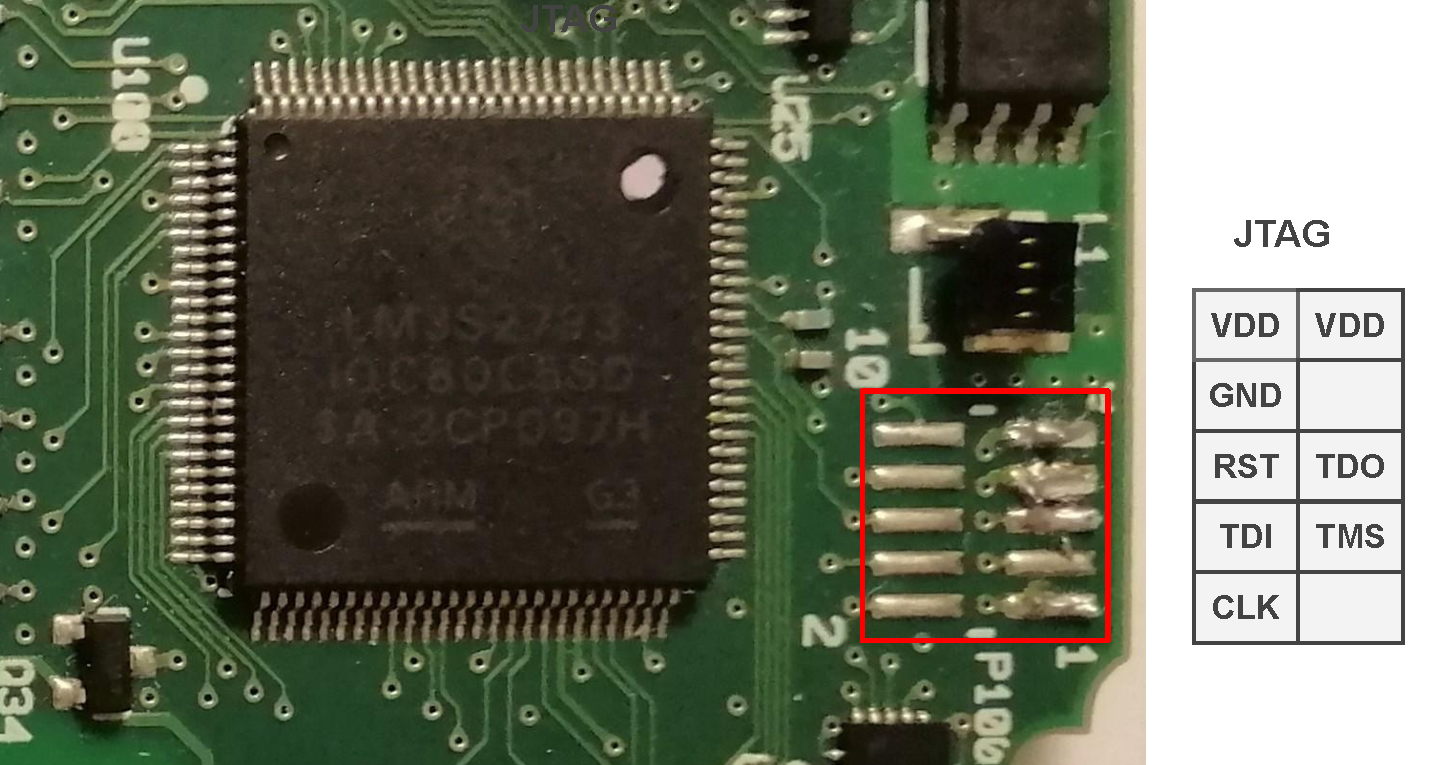
\includegraphics[width=0.47\textwidth]{figures/board_jtag}
	\centering
	\caption{JTAG Interface on the Real-time Microcontroller Board}
	\label{fig:board_jtag}
\end{figure}


\textbf{\textit{JTAG Protocol.}}

We want the hardware backdoor's physical size as small as possible to be less noticeable inside a PLC. Therefore we decide to use a microcontroller soc to achieve the function. It includes a primary JTAG protocol driver and operations on the CoreSight DAP registers, equivalent to a very basic hardware debugger. We can not use open source hardware debugger implementation such as OpenOCD~\cite{hogl2006open} because the soc we choose has a Cortex-M3 core that can not support the runtime environment OpenOCD needs.

We use the Teensy 3.2 development board for its small PCB size, and we implement the JTAG protocol on top of it in a bare-metal runtime environment. The source code is available at the github~\footnote{https://github.com/whensungoesdown/teensy\_jtag}. We call this part the control module for the rest of the paper. 


\textbf{\textit{Remote Control}} is the basic function of a backdoor. Due to the possible network access control that the target network may have deployed, we choose to use a wireless cellular network to send control commands. Therefore an additional GSM module is added to the backdoor and connects with the control module through a serial port.
